% Options for packages loaded elsewhere
\PassOptionsToPackage{unicode}{hyperref}
\PassOptionsToPackage{hyphens}{url}
%
\documentclass[
  ignorenonframetext,
]{beamer}
\usepackage{pgfpages}
\setbeamertemplate{caption}[numbered]
\setbeamertemplate{caption label separator}{: }
\setbeamercolor{caption name}{fg=normal text.fg}
\beamertemplatenavigationsymbolsempty
% Prevent slide breaks in the middle of a paragraph
\widowpenalties 1 10000
\raggedbottom
\setbeamertemplate{part page}{
  \centering
  \begin{beamercolorbox}[sep=16pt,center]{part title}
    \usebeamerfont{part title}\insertpart\par
  \end{beamercolorbox}
}
\setbeamertemplate{section page}{
  \centering
  \begin{beamercolorbox}[sep=12pt,center]{part title}
    \usebeamerfont{section title}\insertsection\par
  \end{beamercolorbox}
}
\setbeamertemplate{subsection page}{
  \centering
  \begin{beamercolorbox}[sep=8pt,center]{part title}
    \usebeamerfont{subsection title}\insertsubsection\par
  \end{beamercolorbox}
}
\AtBeginPart{
  \frame{\partpage}
}
\AtBeginSection{
  \ifbibliography
  \else
    \frame{\sectionpage}
  \fi
}
\AtBeginSubsection{
  \frame{\subsectionpage}
}

\usepackage{amsmath,amssymb}
\usepackage{iftex}
\ifPDFTeX
  \usepackage[T1]{fontenc}
  \usepackage[utf8]{inputenc}
  \usepackage{textcomp} % provide euro and other symbols
\else % if luatex or xetex
  \usepackage{unicode-math}
  \defaultfontfeatures{Scale=MatchLowercase}
  \defaultfontfeatures[\rmfamily]{Ligatures=TeX,Scale=1}
\fi
\usepackage{lmodern}
\ifPDFTeX\else  
    % xetex/luatex font selection
\fi
% Use upquote if available, for straight quotes in verbatim environments
\IfFileExists{upquote.sty}{\usepackage{upquote}}{}
\IfFileExists{microtype.sty}{% use microtype if available
  \usepackage[]{microtype}
  \UseMicrotypeSet[protrusion]{basicmath} % disable protrusion for tt fonts
}{}
\makeatletter
\@ifundefined{KOMAClassName}{% if non-KOMA class
  \IfFileExists{parskip.sty}{%
    \usepackage{parskip}
  }{% else
    \setlength{\parindent}{0pt}
    \setlength{\parskip}{6pt plus 2pt minus 1pt}}
}{% if KOMA class
  \KOMAoptions{parskip=half}}
\makeatother
\usepackage{xcolor}
\newif\ifbibliography
\setlength{\emergencystretch}{3em} % prevent overfull lines
\setcounter{secnumdepth}{-\maxdimen} % remove section numbering


\providecommand{\tightlist}{%
  \setlength{\itemsep}{0pt}\setlength{\parskip}{0pt}}\usepackage{longtable,booktabs,array}
\usepackage{calc} % for calculating minipage widths
\usepackage{caption}
% Make caption package work with longtable
\makeatletter
\def\fnum@table{\tablename~\thetable}
\makeatother
\usepackage{graphicx}
\makeatletter
\def\maxwidth{\ifdim\Gin@nat@width>\linewidth\linewidth\else\Gin@nat@width\fi}
\def\maxheight{\ifdim\Gin@nat@height>\textheight\textheight\else\Gin@nat@height\fi}
\makeatother
% Scale images if necessary, so that they will not overflow the page
% margins by default, and it is still possible to overwrite the defaults
% using explicit options in \includegraphics[width, height, ...]{}
\setkeys{Gin}{width=\maxwidth,height=\maxheight,keepaspectratio}
% Set default figure placement to htbp
\makeatletter
\def\fps@figure{htbp}
\makeatother

\makeatletter
\@ifpackageloaded{caption}{}{\usepackage{caption}}
\AtBeginDocument{%
\ifdefined\contentsname
  \renewcommand*\contentsname{Table of contents}
\else
  \newcommand\contentsname{Table of contents}
\fi
\ifdefined\listfigurename
  \renewcommand*\listfigurename{List of Figures}
\else
  \newcommand\listfigurename{List of Figures}
\fi
\ifdefined\listtablename
  \renewcommand*\listtablename{List of Tables}
\else
  \newcommand\listtablename{List of Tables}
\fi
\ifdefined\figurename
  \renewcommand*\figurename{Figure}
\else
  \newcommand\figurename{Figure}
\fi
\ifdefined\tablename
  \renewcommand*\tablename{Table}
\else
  \newcommand\tablename{Table}
\fi
}
\@ifpackageloaded{float}{}{\usepackage{float}}
\floatstyle{ruled}
\@ifundefined{c@chapter}{\newfloat{codelisting}{h}{lop}}{\newfloat{codelisting}{h}{lop}[chapter]}
\floatname{codelisting}{Listing}
\newcommand*\listoflistings{\listof{codelisting}{List of Listings}}
\makeatother
\makeatletter
\makeatother
\makeatletter
\@ifpackageloaded{caption}{}{\usepackage{caption}}
\@ifpackageloaded{subcaption}{}{\usepackage{subcaption}}
\makeatother

\ifLuaTeX
  \usepackage{selnolig}  % disable illegal ligatures
\fi
\usepackage{bookmark}

\IfFileExists{xurl.sty}{\usepackage{xurl}}{} % add URL line breaks if available
\urlstyle{same} % disable monospaced font for URLs
\hypersetup{
  pdftitle={Exchange rate I: the monetary approach in the long run},
  pdfauthor={I Made Krisna Gupta},
  hidelinks,
  pdfcreator={LaTeX via pandoc}}


\title{Exchange rate I: the monetary approach in the long run}
\subtitle{ECES905205 pertemuan 3}
\author{I Made Krisna Gupta}
\date{2024-09-12}

\begin{document}
\frame{\titlepage}


\begin{frame}{Goals}
\phantomsection\label{goals}
\begin{itemize}
\item
  We set out long-run relationships between money, prices and exchange
  rates.
\item
  Two parts of development:

  \begin{itemize}
  \item
    Purchasing power, linking exchange rate and prices in different
    countries.
  \item
    Linking price levels and monetary conditions in each countries.
  \end{itemize}
\item
  Combination of the two: the monetary approach to exchange rates.
\end{itemize}
\end{frame}

\begin{frame}{Purchasing power parity}
\phantomsection\label{purchasing-power-parity}
\begin{itemize}
\item
  Since goods can be traded, arbitrage can happen, thus prices can
  converge in the international market.
\item
  Applied to a single good, we call this ``law of one price'' (LOOP).
\item
  Applied to a basket of goods, we call this ``purchasing power
  parity''.
\item
  We start by assuming a frictionless trade (no trade cost).
\end{itemize}
\end{frame}

\begin{frame}{LOOP}
\phantomsection\label{loop}
With competitive market, flexible prices and zero trade cost, prices of
identical goods sold in different countries should be the same.

For a good \(g\) sold in 2 places:

\[
q^g_{ID/US}=E_{Rp/\$}\frac{P^g_{US}}{P^g_{ID}}
\]

Where \(q^g_{ID/US}\) is the relative price of good \(g\) in Indonesia
vs the US. Loop is hold if \(q^g_{ID/US}=1\).
\end{frame}

\begin{frame}{LOOP}
\phantomsection\label{loop-1}
If LOOP is hold, we can rearrange the equation above to get:

\[
E_{Rp/\$}P_{US}^{ID}=P^g_{US}
\]

which means the exchange rate must be equal to the ratio of prices
expressed in two currencies.

\[
E_{Rp/\$}=\frac{P_{ID}}{P_{US}}
\]
\end{frame}

\begin{frame}{Purchasing power parity}
\phantomsection\label{purchasing-power-parity-1}
\begin{itemize}
\tightlist
\item
  PPP is the macroeconomic version of LOOP. We compute two basket of
  goods in each location, find their local prices, and compare them.
\end{itemize}

\[
q_{ID/US}=E_{Rp/\$}\frac{P_{US}}{P_{ID}}
\]

\begin{itemize}
\item
  If there are no arbitrage, then the same basket of goods in two
  countries should have the same price. i.e.,\(q_{ID/US}=1\)
\item
  PPP thus holds: price levels in two countries are equal when expressed
  in common currency. This is called absolute PPP.
\end{itemize}
\end{frame}

\begin{frame}{Real exchange rate}
\phantomsection\label{real-exchange-rate}
\begin{itemize}
\item
  The real exchange rate is the relative price of the baskets.
\item
  The Indonesian real exchange rate \(q_{ID/US}=E_{Rp/\$}P_{US}/P_{ID}\)
  tells us how many Indonesian baskets are needed to purchase U.S.
  basket.
\item
  The exchange rate for currencies is a nominal concept. The real
  exchange rate is the real concept.
\item
  The apreciation and depreciation terminology is the same, but add
  real: real appreciation (if \(q \downarrow\)) and real depreciation
  (if \(q \uparrow\)).
\end{itemize}
\end{frame}

\begin{frame}{PPP and exchange rate}
\phantomsection\label{ppp-and-exchange-rate}
\begin{itemize}
\item
  PPP is holding if \(q_{ID/US}=1\), and no incentive to do arbitrage.
\item
  If \(q_{ID/US}>1\), then the Indonesian basket is more expensive than
  the U.S. basket. This means the Rp is overvalued.
\item
  if \(q_{ID/US}<1\), then the Indonesian basket is cheaper than the
  U.S. basket. This means the Rp is undervalued.
\end{itemize}
\end{frame}

\begin{frame}{PPP and exchange rate}
\phantomsection\label{ppp-and-exchange-rate-1}
\begin{itemize}
\tightlist
\item
  When \(q_{ID/US}=1\), then:
\end{itemize}

\begin{equation}
\underbrace{E_{Rp/\$}}_{\text{exchange rate}}=\underbrace{P_{ID}/P_{US}}_\text{ratio of price levels}
\end{equation}

\emph{Purchasing power parity implies that the exchange rate at which
two currencies trade equals the relative price levels of the two
countries.}
\end{frame}

\begin{frame}{Long-run relationship}
\phantomsection\label{long-run-relationship}
\begin{itemize}
\item
  We have established that \(E_{Rp/\$}=P_{ID}/P_{US}\)
\item
  Left-hand side: Let's take a rate of change of the exchange rate
  (i.e., rate of depreciation/appreciation).
\end{itemize}

\begin{equation}
\frac{\Delta E_{Rp/\$}}{E_{Rp/\$}}=\frac{\Delta P_{ID}}{P_{ID}}-\frac{\Delta P_{US}}{P_{US}}
\end{equation}
\end{frame}

\begin{frame}{Long-run relationship}
\phantomsection\label{long-run-relationship-1}
Right-hand side: We do the same, taking growth rate of the price ratio:

\begin{align*}
\frac{\Delta (P_{ID}/P_{US})}{P_{ID}/P_{US}}&=\frac{\Delta P_{ID,t}}{P_{ID,t}}-\frac{\Delta P_{US,t}}{P_{US,t}} \\
&=\left(\frac{P_{ID,t+1}-P_{ID,t}}{P_{ID,t}}\right)-\left(\frac{P_{US,t+1}-P_{US,t}}{P_{US,t}}\right) \\
&=\pi_{ID,t}-\pi_{US,t}\\

\end{align*}
\end{frame}

\begin{frame}{XR and inflation}
\phantomsection\label{xr-and-inflation}
\begin{itemize}
\tightlist
\item
  If \(q_{Rp/\$}=1\), then we have:
\end{itemize}

\begin{equation}
\frac{\Delta E_{Rp/\$,t}}{E_{Rp/\$,t}}=\pi_{ID,t}-\pi_{US,t}
\end{equation}

This is what we call \emph{relative PPP}, which implies that the rate of
depreciation of the nominal exchange rate equals the difference between
the inflation rates of two countries.
\end{frame}

\begin{frame}{Application}
\phantomsection\label{application}
\begin{figure}[H]

{\centering 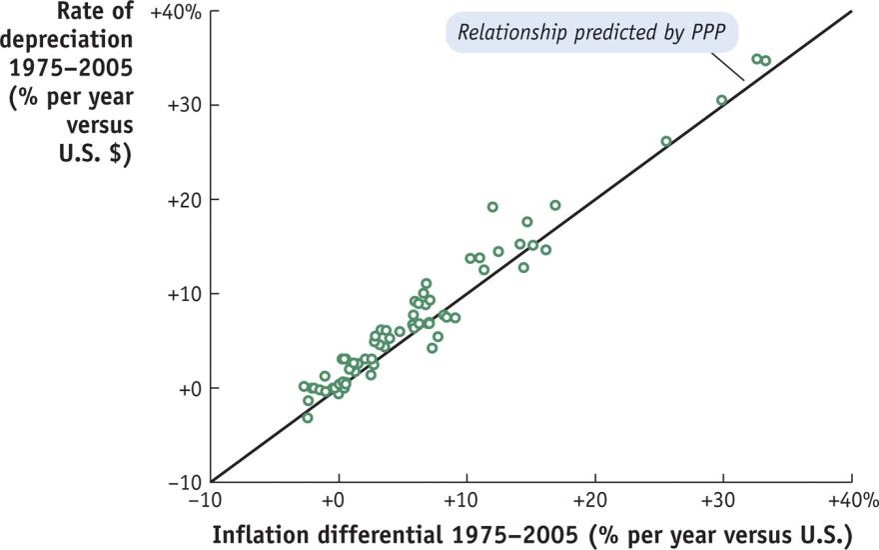
\includegraphics{Picture1.jpg}

}

\caption{The diagonal line expresses rate of depreciation against USD to
be equal with inflation differential against US inflation. Not all align
perfectly with the line, but shows a long-run tendecy of both to be very
close}

\end{figure}%
\end{frame}

\begin{frame}{Application}
\phantomsection\label{application-1}
\begin{figure}[H]

{\centering 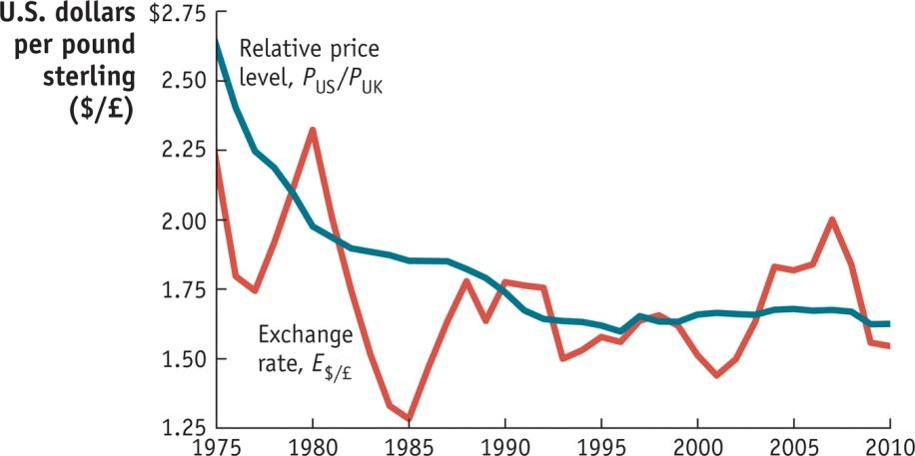
\includegraphics{Picture2.jpg}

}

\caption{Likewise, US/UK exchange rate versus relative price. The two
has tendency to move the same direction and to be equal. Not precisely
all the time but shows a tendency towards equality.}

\end{figure}%
\end{frame}

\begin{frame}{Indonesia?}
\phantomsection\label{indonesia}
What do you think about Indonesia?

\begin{figure}

\begin{minipage}{0.50\linewidth}

\begin{figure}[H]

{\centering 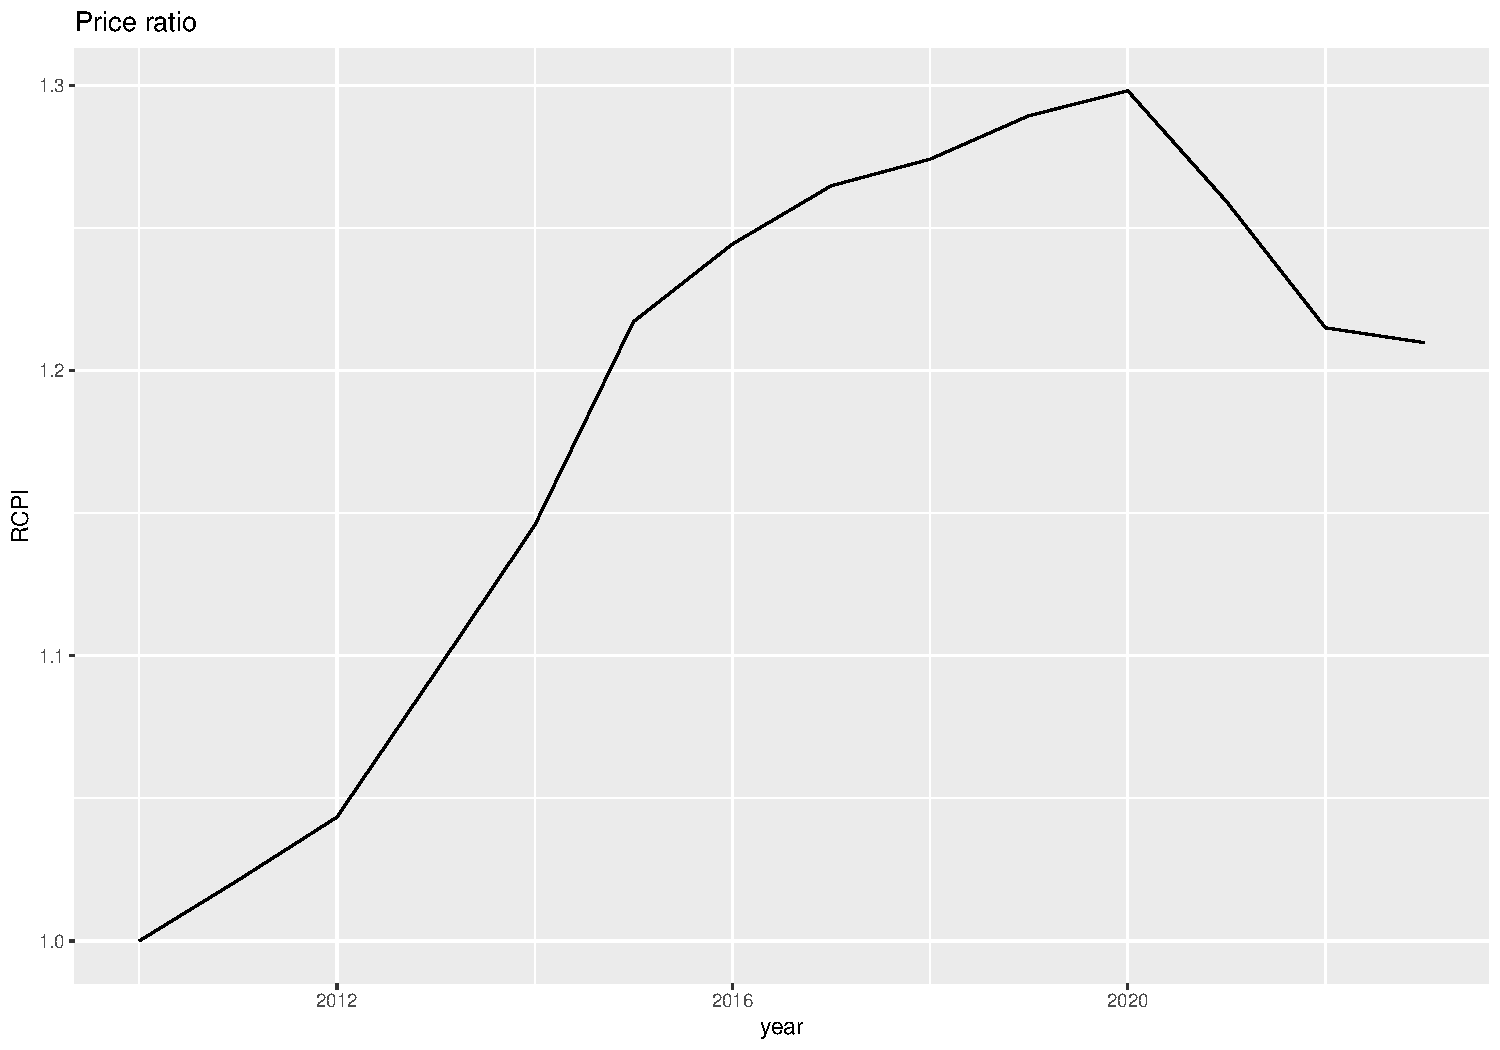
\includegraphics{index_files/figure-beamer/unnamed-chunk-1-1.pdf}

}

\subcaption{Price ratio}

\end{figure}%

\end{minipage}%
%
\begin{minipage}{0.50\linewidth}

\begin{figure}[H]

{\centering 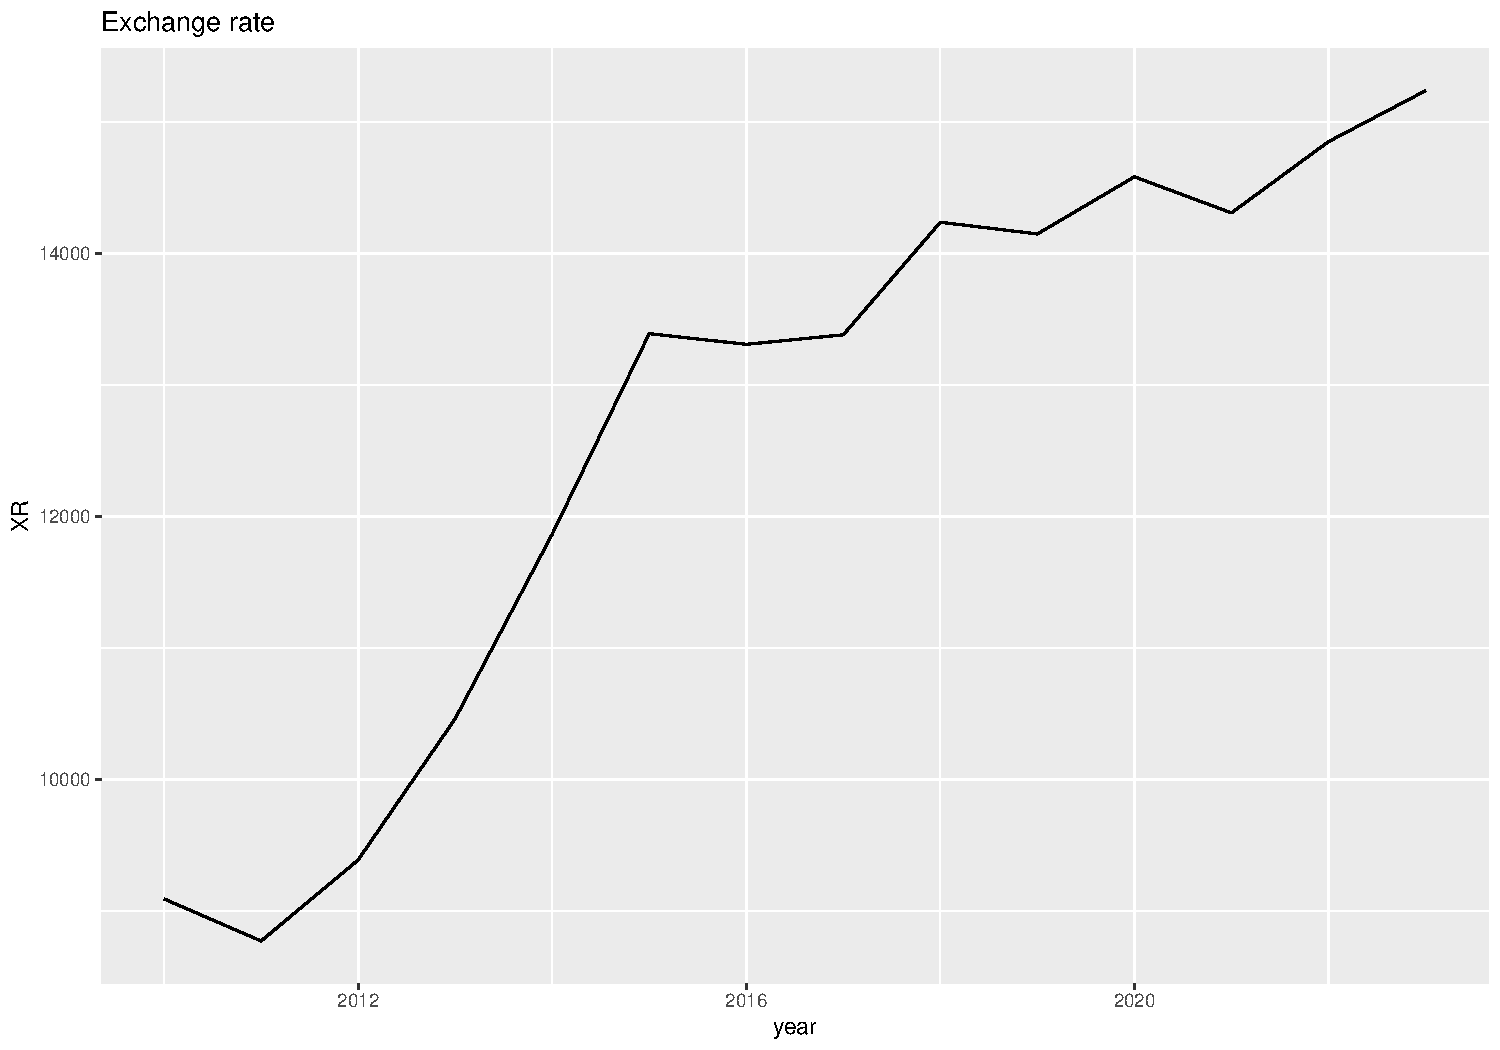
\includegraphics{index_files/figure-beamer/unnamed-chunk-1-2.pdf}

}

\subcaption{Official exchange rate (Rp/\$)}

\end{figure}%

\end{minipage}%

\end{figure}%
\end{frame}

\begin{frame}{Slow convergence}
\phantomsection\label{slow-convergence}
\begin{itemize}
\item
  Research shows that price differences---the deviations from PPP---can
  be quite persistent.
\item
  Estimates suggest that these deviations may die out at a rate of about
  15\% per year. This kind of measure is often called a speed of
  convergence.
\item
  Approximately half of any PPP deviation still remains after four
  years: Economists refer to this as a four-year half-life.
\item
  Such estimates provide a rule of thumb that is useful as a guide to
  forecasting real exchange rates.
\end{itemize}
\end{frame}

\begin{frame}{Forecasting overvaluation}
\phantomsection\label{forecasting-overvaluation}
\begin{itemize}
\tightlist
\item
  When PPP doesn't hold (which often the case), knowing the real
  exchange rate and the convergence speed may still allow us to
  construct a forecast of real and nominal exchange rate.
\end{itemize}

\begin{equation}
\frac{\Delta E_{Rp/\$,t}}{E_{Rp/\$,t}}=\frac{\Delta q_{Rp/\$,t}}{q_{Rp/\$,t}}+\pi_{ID,t}-\pi_{US,t}
\end{equation}
\end{frame}

\begin{frame}{Why PPP doesn't hold}
\phantomsection\label{why-ppp-doesnt-hold}
\begin{itemize}
\item
  Transaction cost, like cost of transportaton, tariffs and
  nnon-tariffs, other shipping cost and delays amid red tape. On
  average, these costs are about 20\% of the goods' price.
\item
  Non-traded goods. Some goods are just non-traded. We can think of it
  as infinitely high transaction cost. Most goods are falling between
  perfectly tradable and non-tradable.
\end{itemize}
\end{frame}

\begin{frame}{Why PPP doesn't hold}
\phantomsection\label{why-ppp-doesnt-hold-1}
\begin{itemize}
\item
  Price stickiness. Prices are sticky, and it takes time for prices to
  adjust. This is especially true for services, which are more difficult
  to trade.
\item
  Imperfect competition. Firms may have market power, and thus can
  charge different prices in different markets.
\end{itemize}
\end{frame}

\begin{frame}{Big Mac Index}
\phantomsection\label{big-mac-index}
For more than 25 years,
\href{https://www.krisna.or.id/post/bigmacindex/}{The Economist
newspaper} has engaged in a whimsical attempt to judge PPP theory based
on a well-known, globally uniform consumer good: the McDonald's Big Mac.
The over- or undervaluation of a currency against the U.S. dollar is
gauged by comparing the relative prices of a burger in a common
currency, and expressing the difference as a percentage deviation from
one:

\begin{equation}
\text{Big Mac Index}=q^{\text{Big Mac}}-1=\left(\frac{E_{\$/lc}P^{Bigmac}_local}{P_{US}^{Bigmac}}\right)-1
\end{equation}
\end{frame}

\begin{frame}{Monetary theory}
\phantomsection\label{monetary-theory}
\begin{itemize}
\item
  Exchange rates determined by price ratio of two countries, but what
  determines those prices?
\item
  Monetary theory: in the long run, price levels are determined in each
  country by the relative demand and supply of money.
\end{itemize}
\end{frame}

\begin{frame}{What is money?}
\phantomsection\label{what-is-money}
Stuff that serves these 3 functions:

\begin{enumerate}
\item
  Money is a store of value because it can be used to buy goods and
  services in the future. If the opportunity cost of holding money is
  low, we will hold money more willingly than we hold other assets.
\item
  Money also gives us a unit of account in which all prices in the
  economy are quoted.
\item
  Money is a medium of exchange that allows us to buy and sell goods and
  services without the need to engage in inefficient barter.
\end{enumerate}
\end{frame}

\begin{frame}{Money demand}
\phantomsection\label{money-demand}
\begin{itemize}
\tightlist
\item
  A simple model of money demand: we want to hold money when we want to
  have a transaction. The more nominal income (PY), the more money we
  want to hold. Adding a constant multiplier \(\bar{L}\):
\end{itemize}

\begin{equation}
M^d=\bar{L}PY
\end{equation}

Real money demand thus:

\begin{equation}
\frac{M^d}{P}=\bar{L}Y
\end{equation}
\end{frame}

\begin{frame}{Money market equilibrium}
\phantomsection\label{money-market-equilibrium}
\begin{itemize}
\item
  In the equilibrium, money demand = money supply \(M_d=M\). M is
  exogenous because we assume it's fully controlled by the central bank.
\item
  Therefore, \(M=\bar{L}PY\), which means in the equilibrium:
\end{itemize}

\begin{equation}
\frac{M}{P}=\bar{L}Y
\end{equation}
\end{frame}

\begin{frame}{Simple price model}
\phantomsection\label{simple-price-model}
\begin{itemize}
\tightlist
\item
  Since ID and US has their own market, thus 2 prices, then
\end{itemize}

\begin{equation}
P_{ID}=\frac{M_{ID}}{\bar{L}Y_{ID}} \quad \text{and} \quad P_{US}=\frac{M_{US}}{\bar{L}Y_{US}}
\end{equation}

\begin{itemize}
\item
  These twoequationns are examples of the fundamental equation of the
  monetary model of the price level.
\item
  In the long run, we assume prices are flexible and will adjust to put
  the money market in equilibrium.
\end{itemize}
\end{frame}

\begin{frame}{Money, Prices, XR}
\phantomsection\label{money-prices-xr}
We use our absolute PPP to solve for the exchange rate:

\begin{align*}
E_{Rp/\$}&=\frac{P_{ID}}{P_{US}}=\frac{\left(\frac{M_{ID}}{\bar{L}_{ID}Y_{ID}}\right)}{\left(\frac{M_{US}}{\bar{L}_{US}Y_{US}}\right)} \\
E_{Rp/\$}&=\frac{M_{ID}/M_{US}}{\bar{L}_{ID}Y_{ID}/\bar{L}_{US}Y_{US}}
\end{align*}

This is the fundamental equation of the monetary approach to exchange
rates.
\end{frame}

\begin{frame}{M, P, XR}
\phantomsection\label{m-p-xr}
\begin{equation}
E_{Rp/\$}=\frac{P_{ID}}{P_{US}}\frac{M_{ID}/M_{US}}{\bar{L}_{ID}Y_{ID}/\bar{L}_{US}Y_{US}}
\end{equation}

Say ID's money supply goes up, all else equal. The right handside
equation increases, thus ID's price goes up relative to the US, thus E
goes up (IDR depreciate against USD)

Suppose ID real income goes up, IDR will appreciate. Can you explain
why?
\end{frame}

\begin{frame}{M, P, XR growth}
\phantomsection\label{m-p-xr-growth}
We use similar approach as befre using growth, where growth of money
supply and real income are expressed as follows:

\begin{align*}
\mu_{ID,t}&=\frac{M_{ID,t+1}-M_{ID,t}}{M_{ID}} \\
g_{ID,t}&=\frac{Y_{ID,t+1}-Y_{ID,t}}{Y_{ID}}
\end{align*}
\end{frame}

\begin{frame}{M, P, XR growth}
\phantomsection\label{m-p-xr-growth-1}
Therefore, the growth rate of \(P_{ID}=M_{ID}/\bar{L}_{ID}Y_{ID}\)
equals the money supply growth rate \(\mu_{ID}\) minus the real income
growth rate \(g_{ID}\) (\(\bar{L}\) is gone. why?)

Growth rate of \(P_{i}\) is an inflation rate \(\pi_{i}\), we get:

\begin{align*}
\text{in ID:} \pi_{ID,t}&=\mu_{ID,t}-g_{ID,t} \\
\text{in US:} \pi_{US,t}&=\mu_{US,t}-g_{US,t}
\end{align*}

\emph{When money growth is higher than income growth, we have ``more
money chasing fewer goods'' and this leads to inflation.}
\end{frame}

\begin{frame}{M, P, XR growth}
\phantomsection\label{m-p-xr-growth-2}
Combining the two, we get:

\begin{align*}
\frac{\Delta E_{Rp/\$,t}}{E_{Rp/\$,t}}&=\pi_{ID,t}-\pi_{US,t} \\
&= (\mu_{ID,t}-g_{ID,t})-(\mu_{US,t}-g_{US,t}) \\
\end{align*}

XR depreciation reflects a differece of two countries' money growth and
growth rate.
\end{frame}

\begin{frame}{M,P,depreciation}
\phantomsection\label{mpdepreciation}
\begin{align*}
\frac{\Delta E_{Rp/\$,t}}{E_{Rp/\$,t}}&=\pi_{ID,t}-\pi_{US,t} \\
&= (\mu_{ID,t}-g_{ID,t})-(\mu_{US,t}-g_{US,t}) \\
\end{align*}

If ID runs a looser monetary policy in the long run, measured by a
faster money growth rate, the Rupiah will depreciate more rapidly,
ceteris paribus.

\begin{itemize}
\tightlist
\item
  If ID growth rate is higher than US in the long run, IDR will
  appreciate more rapidly, ceteris paribus.
\end{itemize}
\end{frame}

\begin{frame}{Forecasting XR}
\phantomsection\label{forecasting-xr}
Using this model, we ask what path would exchange rate follows from now
on if prices were flexible and PPP held?

\begin{itemize}
\item
  Assume ID and US real income growth rates are identical and equal to
  zero (0\%). Also, US price level is constant with zero inflation.
\item
  2 cases: (1) a one-time increase in the money supply, and (2) an
  increase in the rate of money growth.
\end{itemize}
\end{frame}

\begin{frame}{Case 1}
\phantomsection\label{case-1}
\begin{itemize}
\item
  There is a 10\% increase in the money supply M.
\item
  Real money balances M/P remain constant because real income is
  constant.
\item
  These previous two statements imply that price level P and money
  supply M must move in the same proportion, so there is a 10\% increase
  in the price level P.
\item
  PPP implies that the exchange rate E and price level P must move in
  the same proportion, so there is a 10\% increase in the exchange rate
  E.
\end{itemize}
\end{frame}

\begin{frame}{Case 2}
\phantomsection\label{case-2}
At time T the Indonesia will raise the rate of money supply growth to
rate of μ + Δμ from a steady fixed rate μ.

\begin{itemize}
\item
  Money supply M is growing at a constant rate.
\item
  Real money balances M/P remain constant, as before.
\item
  These previous two statements imply that price level P and money
  supply M must move in the same proportion, so P is always a constant
  multiple of M.
\item
  PPP implies that the exchange rate E and price level P must move in
  the same proportion, so E is always a constant multiple of P (and
  hence of M).
\end{itemize}
\end{frame}

\begin{frame}{Application}
\phantomsection\label{application-2}
\begin{figure}[H]

{\centering 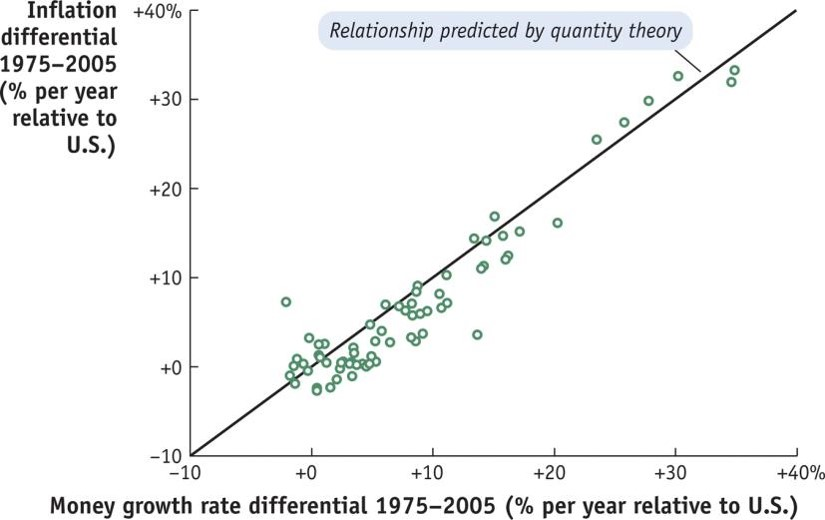
\includegraphics{Picture3.jpg}

}

\caption{It shows the relationship between rate of inflation rate and
money growth differential relative to the US. The line reflects
equality. Not exactly the same but very close.}

\end{figure}%
\end{frame}

\begin{frame}{Applicationn}
\phantomsection\label{applicationn}
\begin{figure}[H]

{\centering 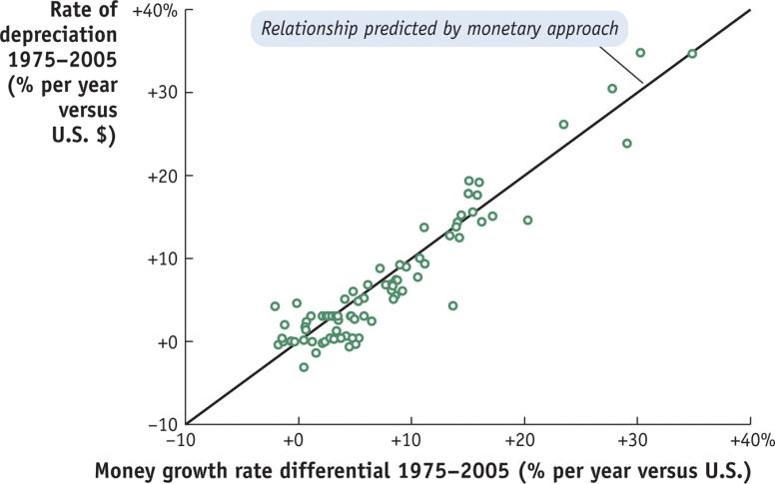
\includegraphics{Picture4.jpg}

}

\caption{It shows the relationship between rate of exchange rate
depreciation and money growth differential relative to the US. The line
reflects equality. Not exactly the same but very close.}

\end{figure}%
\end{frame}

\begin{frame}{Hyperinflation}
\phantomsection\label{hyperinflation}
The monetary approach assumes long-run PPP, which generally works poorly
in the short run. There is one notable exception to this general failure
of PPP in the short run: hyperinflation.

\begin{itemize}
\item
  Economists traditionally define a hyperinflation as a sustained
  inflation of more than 50\% per month (which means that prices are
  doubling every 51 days).
\item
  In common usage, some lower-inflation episodes are also called
  hyperinflations. An inflation rate of 1,000\% per year is a common
  rule of thumb (22\% per month).
\item
  Hyperinflations usually occur when governments face a budget crisis,
  are unable to borrow to finance a deficit, and instead choose to print
  money.
\end{itemize}
\end{frame}

\begin{frame}{Zimbabwe case}
\phantomsection\label{zimbabwe-case}
By 2007 Zimbabwe was almost at an economic standstill, except for the
printing presses churning out the banknotes. - A creeping
inflation---58\% in 1999, 132\% in 2001, 385\% in 2003, and 586\% in
2005---was about to become hyperinflation, and the long-suffering people
faced an accelerating descent into even deeper chaos. - By 2007
inflation had risen to 12,000\%! - This was one the five worst
hyperinflations of all time. - In 2008, the local currency disappeared
from use, replaced by U.S. dollars and South African rand.
\end{frame}

\begin{frame}[s]{Currency reform}
\phantomsection\label{currency-reform}
Currencies can become extinct if they cease to function well and lose
value rapidly (e.g., dollarization in Ecuador). If the currency
survives, the government may redenominate a new currency unit equal to
10N (10 to the power N) old units. Sometimes N can get quite
large\ldots.

\begin{itemize}
\tightlist
\item
  In the 1980s, Argentina suffered hyperinflation. In June 1983, the
  peso argentino replaced the (old) peso at a rate of 10,000 to 1. In
  June 1985, the austral replaced the peso argentino at 1,000 to 1.
  Finally, in January 1992, the convertible peso replaced the austral at
  a rate of 10,000 to 1 (i.e., 10,000,000,000 old pesos).
\item
  In 1946, the Hungarian pengö became worthless. By July 15, 1946, there
  were 76,041,000,000,000,000,000,000,000 pengö in circulation.
\end{itemize}
\end{frame}

\begin{frame}{General model}
\phantomsection\label{general-model}
\begin{itemize}
\item
  We assume a stable demand of money, and it's not necessarily true.
\item
  We will now explore a more general model that allows for money demand
  to vary with the nominal interest rate.
\item
  We consider the links between inflation and the nominal interest rate
  in an open economy.
\item
  We then return to the question of how best to understand what
  determines exchange rates in the long run.
\end{itemize}
\end{frame}

\begin{frame}{General model}
\phantomsection\label{general-model-1}
\begin{itemize}
\item
  Suppose the demand for money depends on interest rate: high interest
  rate makes holding money expensive. This makes \(\bar{L}\) no longer
  constant.
\item
  L is a decreasing function of the nominal interest rate \(i\)
\end{itemize}

\begin{equation}
M^d=L(i_{Rp})PY \rightarrow \frac{M^d}{P}=L(i_{Rp})Y
\end{equation}
\end{frame}

\begin{frame}{M and i}
\phantomsection\label{m-and-i}
\begin{figure}[H]

{\centering 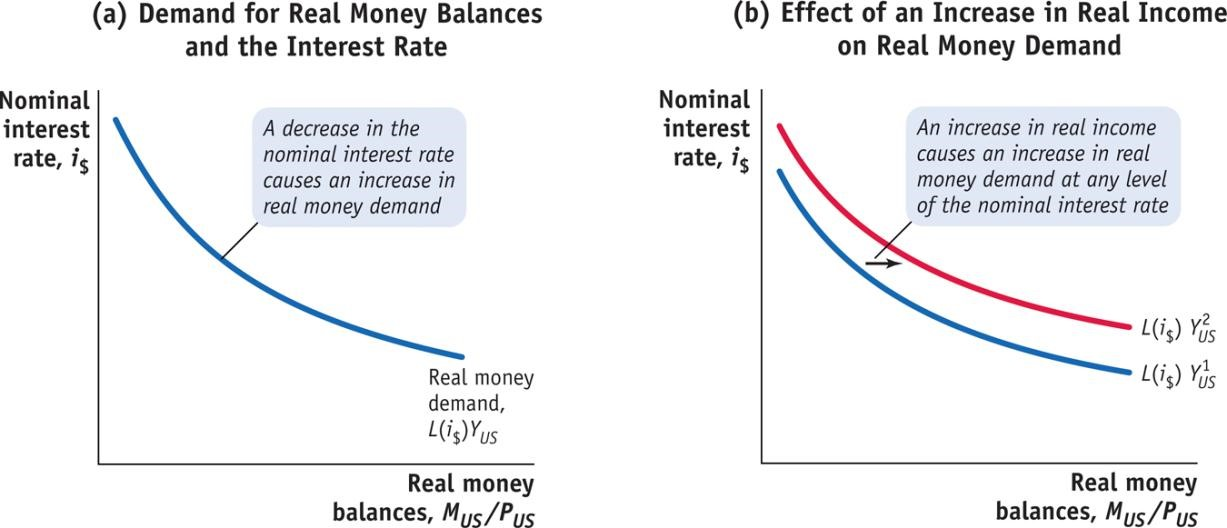
\includegraphics{Picture5.jpg}

}

\caption{The higher innterest rate, the lower money demand is. An
increase in real income will shifts the curve to the right}

\end{figure}%
\end{frame}

\begin{frame}{General model}
\phantomsection\label{general-model-2}
Money market long-run equilibrium (\(M=M^d\))

\begin{equationn}
\frac{M}{P}=L(i)Y
\end{equationn}

With this relationship and PPP and UIP holds, we can derive the long-run
exchange rate depretiation.

\begin{equation}
\frac{\Delta E^e_{Rp/\$,t}}{E_{Rp/\$,t}}=\pi^e_{ID,t}-\pi^e_{US,t} \ \text{and} \ \frac{\Delta E^e_{Rp/\$,t}}{E_{Rp/\$,t}}=i_{Rp,t}-i_{US,t}
\end{equation}
\end{frame}

\begin{frame}{The fisher effect}
\phantomsection\label{the-fisher-effect}
Therefore, we have that inflation expectation difference is equal to
nominal interest rate difference.

\begin{equation}
\pi^e_{ID,t}-\pi^e_{US,t} = i_{Rp,t}-i_{US,t}
\end{equation}

All else equal, a rise in the expected inflation rate in a country will
lead to an equal rise in its nominal interest rate. This is called the
fisher effect.

Fisher effect predicts that the change in the opportunity cost of money
is equal not just to the change in the nominal interest rate but also to
the change in the inflation rate.
\end{frame}

\begin{frame}{Real interest parity}
\phantomsection\label{real-interest-parity}
\begin{itemize}
\tightlist
\item
  rearranging the previous equation gets us
\end{itemize}

\begin{equation}
i_{Rp,t}-\pi^e_{ID,t} = i_{US,t}-\pi^e_{US,t}
\end{equation}

\begin{itemize}
\tightlist
\item
  subtracting th einflation rate from the nominal interest rate gives us
  \emph{real interest rate} (r), the inflation-adjusted return on an
  interest-bearing asset.
\end{itemize}

\begin{equation}
r^e_{ID}=r^e_{US}
\end{equation}
\end{frame}

\begin{frame}{Real interest parity}
\phantomsection\label{real-interest-parity-1}
The condition is called real interest parity:

\emph{If PPP and UIP hold, then nexpected real interest rates are
equalized across countries}

Real interest parity implies that arbitrage in goods (PPP) and financial
markets (UIP) alone in sufficient, in the long run, to cause the
equalization of real interest rates across countries.

Thus, \(r^e_{ID}=r^e_{US}=r^*\)
\end{frame}

\begin{frame}{Real interest parity}
\phantomsection\label{real-interest-parity-2}
We treat \(r^*\) as an exogeneous variable, something no policy maker in
any country can control.

Unnder this condition, the Fisher effect is even clearer because by
definition

\begin{align*}
i_{Rp}=r^e_{ID}+\pi^e_{ID} = r^*+\pi^e_{ID} \\
i_{\$}=r^e_{US}+\pi^e_{US} = r^*+\pi^e_{US}
\end{align*}
\end{frame}

\begin{frame}{Fisher effect evidence}
\phantomsection\label{fisher-effect-evidence}
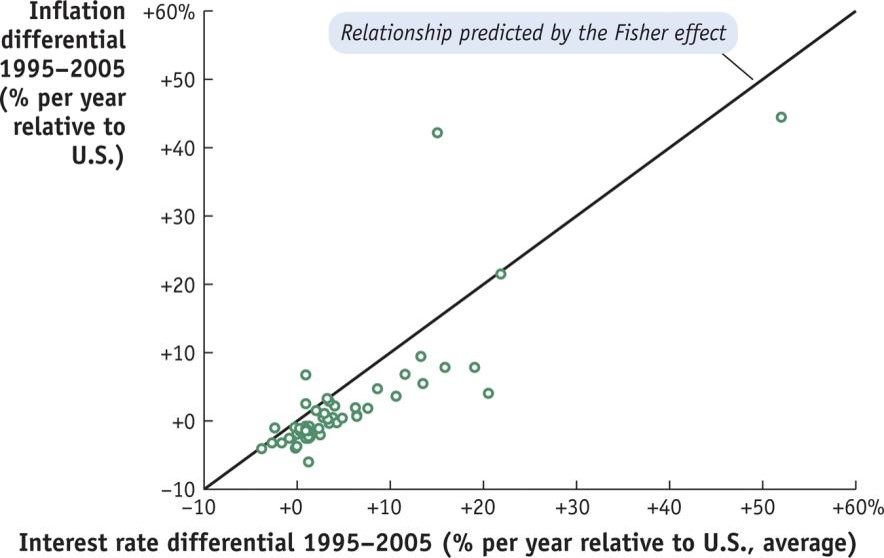
\includegraphics{Picture6.jpg}
\end{frame}

\begin{frame}{General model fundamental}
\phantomsection\label{general-model-fundamental}
Now that money demand moves negatively with interest rate, we can
express exchange rate as:

\begin{equation}
E_{Rp/\$}=\frac{P_{ID}}{P_{US}}\frac{M_{ID}/M_{US}}{L_{ID}(i_{Rp})Y_{ID}/L_{US}(i_\$)Y_{US}}
\end{equation}

Let's reexamine case 2 where Indonesia rises money growth rate from
\(\mu\) to \(\mu+\Delta\mu\).
\end{frame}

\begin{frame}{Case 2 revisited}
\phantomsection\label{case-2-revisited}
At time T the Indonesia will raise the rate of money supply growth to
rate of μ + Δμ from a steady fixed rate μ.

\begin{itemize}
\item
  Money supply M is growing at a constant rate.
\item
  Real money balances M/P remain constant, as before.
\item
  These previous two statements imply that price level P and money
  supply M must move in the same proportion, so P is always a constant
  multiple of M.
\item
  Fisher effect suggests that inflation leads to a same proportion
  changes of interest rate.
\item
  Real money demand thus falls with a discrete jump at time \(T\)
\end{itemize}
\end{frame}

\begin{frame}{Monetary and exchange rate regime}
\phantomsection\label{monetary-and-exchange-rate-regime}
An overarching aspect of a nation's economic policy is the desire to
keep inflation within certain bounds.

\begin{itemize}
\item
  To achieve such an objective requires that policy makers be subject to
  some kind of constraint in the long run. Such constraints are called
  nominal anchors.
\item
  Long-run nominal anchoring and short-run flexibility are the
  characteristics of the policy framework that economists call the
  monetary regime.
\item
  The three main nominal anchor choices that emerge are exchange rate
  target, money supply target, and inflation target plus interest rate
  policy.
\end{itemize}
\end{frame}

\begin{frame}{Exchange rate target:}
\phantomsection\label{exchange-rate-target}
We relabel Indonesia as Home (H) and US as Foreign (F)

\begin{equation}
\pi_H=\underbrace{\frac{\Delta E_{H/F}}{E_{H/F}}}_{text{anchor variable}}+\pi_F
\end{equation}

Relative PPP says that home inflation equals the rate of depreciation
plus foreign inflation. A simple rule would be to set the rate of
depreciation equal to a constant.
\end{frame}

\begin{frame}{Money supply target}
\phantomsection\label{money-supply-target}
\begin{equation}
\pi_H=\mu_H+\g_H
\end{equation}

Simple rule in this case is to set a growth rate of money supply equal
to a constant, say 2\% a year.

The drawback is the final term in the previous equation: real income
growth can be unstable. In periods of high growth, inflation will be
below the desired level. In periods of low growth, inflation will be
above the desired level.
\end{frame}

\begin{frame}{Inflation target}
\phantomsection\label{inflation-target}
combined with interest rate policy as its anchor variable:

\begin{equation}
\pi^e_H=i_H+r^*
\end{equation}

Fisher effect says home inflation is the home nomninal interest rate
minus world interest rate. If the latter is constant and the average
home nominal interest rate is stable, inflation can be kept stable. But
the target nominnal rate must be adjusted if the world real interest
rate changes, as recently happend.
\end{frame}

\begin{frame}[s]{Anchoring}
\phantomsection\label{anchoring}
\begin{figure}[H]

{\centering 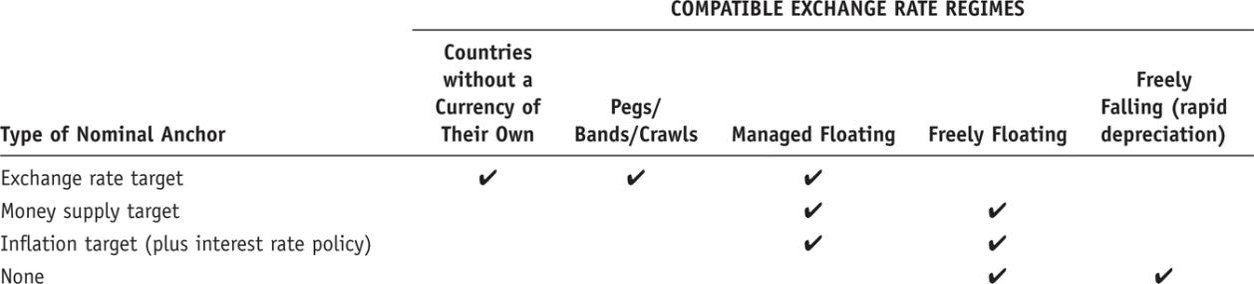
\includegraphics{Picture7.jpg}

}

\caption{This table illustrates the possible exchange rate regimes that
are consistent with various types of nominal anchors. Countries that are
dollarized or in a currency union have a ``superfixed'' exchange rate
target. Pegs, bands, and crawls also target the exchange rate. Managed
floats have no preset path for the exchange rate, which allows other
targets to be employed. Countries that float freely or independently are
judged to pay no serious attention to exchange rate targets; if they
have anchors, they will involve monetary targets or inflation targets
with an interest rate policy. The countries with ``freely falling''
exchange rates have no serious target and have high rates of inflation
and depreciation}

\end{figure}%
\end{frame}

\begin{frame}{Nominal anchoring}
\phantomsection\label{nominal-anchoring}
\begin{itemize}
\item
  An appreciation of the importance of nominal anchors has transformed
  monetary policy making and inflation performance throughout the global
  economy in recent decades.
\item
  In the 1970s and 1980s, most of the world was struggling with high
  inflation.
\item
  In the 1990s, policies designed to create effective nominal anchors
  were put in place in many countries.
\item
  Most of those policies have turned out to be credible, too, thanks to
  political developments in many countries that have fostered
  central-bank independence.
\end{itemize}
\end{frame}




\end{document}
